\section{Scelta della camera}
Nel capitolo precedente è stato illustrato un metodo atto all'identificazione delle frecce che rientrano nel campo visivo della camera. Viene ora trattato come sia possibile ottenere la posizione della freccia, precedentemente ottenuta, nelle coordinate 3D XYZ rispetto alla base del robot.



\begin{figure}
	\centering
	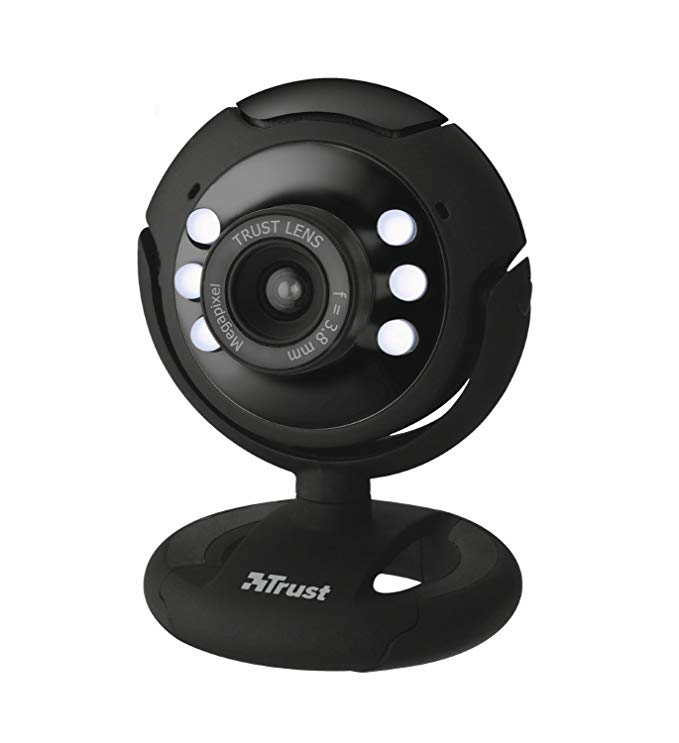
\includegraphics[width=0.5\textwidth]{Immagini/TrustCam.jpg}
	\caption{Camera utilizzata inizialmente}
	\label{fig:TrustCam}
\end{figure}


\section{Vericale o orizzontale?}
\section{Come ottenere le immagini dalla camera?}
